\documentclass{article}[8pt]
\usepackage{textcomp}
\usepackage{geometry}[margin=1inch]
\usepackage{float}
\usepackage{fancyhdr}
\usepackage{listings}
\usepackage{titlesec}
\usepackage{titling}
\usepackage{hyperref}
\usepackage{amsmath}
\usepackage{amsfonts}
\usepackage{mathtools}
\usepackage{sectsty}

\DeclareMathSizes{8}{8}{6}{6}

\lstset{breaklines=true}
\hypersetup{
        colorlinks=true,
        linkcolor=blue,
        filecolor=magenta,
        urlcolor=blue,
        citecolor=blue,
	anchorcolor=blue
}
\title{\vspace{-2cm}SFWRENG-3BB4 Assignment 1\vspace{-.3cm}}
\author{Matthew Farah, \href{mailto:farahm11@mcmaster.ca}{$\langle$farahm11@mcmaster.ca$\rangle$}, 400468251}
\date{\today}
\renewcommand{\thesubsubsection}{\thesection.\alph{subsection}.\Roman{subsubsection}}
\makeatletter
\renewcommand{\thesubsection}{\thesection.\alph{subsection}}

\sectionfont{\fontsize{12}{12}\bfseries}
\subsectionfont{\fontsize{10}{12}\normalfont}
\subsubsectionfont{\fontsize{10}{12}\normalfont}

\pagestyle{fancy}
\fancyhead{}
\fancyhead[L]{Matthew Farah, $\langle$\href{mailto:farahm11@mcmaster.ca}{farahm11@mcmaster.ca}$\rangle$, 400468251}
\fancyhead[R]{\today}

\begin{document}
\maketitle

\begin{center}
	Note that all code Java and LTS code is provided at the end in an appendix
\end{center}

\section[Question ~\thesection]{Consider the following simple hotel reservation system. A customer makes a request for a room. If a room is available, a confirmation is sent to the customer, otherwise, the customer is put on a reservation list. If a room has been confirmed, the customer may either use it, pay for the room, and leave with the whole transaction being archived. However, the customer may also cancel their reservation. When a customer is on the waiting list a room may become available, in which case a confirmation is sent to the customer. The customer may also give up on waiting and cancel their reservation. Model this reservation system as a Finite State Process (FSP). Note that this process always stops, so you must include a STOP process. Also, provide an appropriate Labelled Transition System (LTS) using an LTSA tool.}

\subsection{}

\subsubsection[~\thesubsubsection]{FSP Description}

\begin{align*}
	\text{REQUEST} &= (\text{room\_available} \rightarrow \text{confirm} \rightarrow \text{CHOICE} \; | \; \text{room\_unavailable} \rightarrow \text{WAITLIST}) \\
	\text{CHOICE} &= (\text{use} \rightarrow \text{pay} \rightarrow \text{leave} \rightarrow \text{archive} \rightarrow \text{STOP} \; | \; \text{cancel} \rightarrow \text{STOP}) \\
	\text{WAITLIST} &= (\text{room\_available} \rightarrow \text{confirm} \rightarrow \text{CHOICE} \; | \; \text{room\_unavailable} \rightarrow \text{WAIT}) \\
	\text{WAIT} &= (\text{cancel} \rightarrow \text{STOP} \; | \; wait \text{WAITLIST})
\end{align*}

\subsubsection[~\thesubsubsection]{LTS Representation}

\begin{figure}[H]
	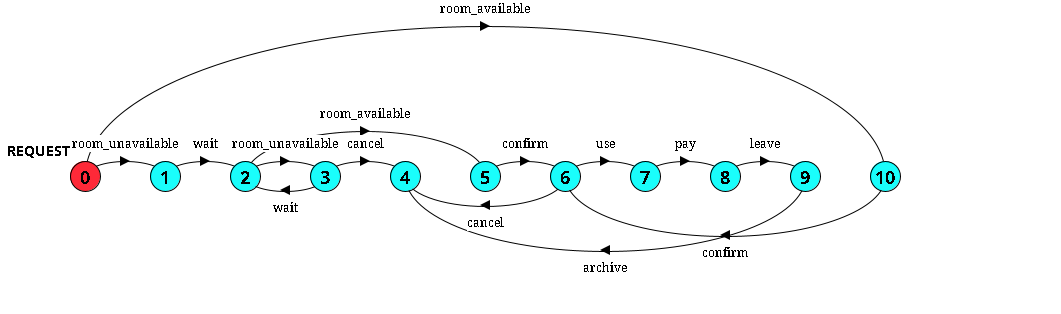
\includegraphics[width=\linewidth]{./imgs/Question-1.png}
	\caption{LTS produced by LTSA tool for Question 1}
	\label{fig:Question-1-LTS}
\end{figure}

\section[Question ~\thesection]{Consider the following three processes:}

\begin{figure}[H]
	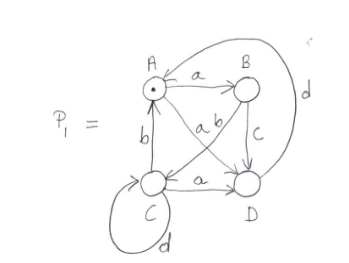
\includegraphics{./imgs/Question-2-a-i.png}
	\caption{Question 2-a LTS 1}
	\label{fig:Question-2-a-i-LTS}
\end{figure}

\begin{figure}[H]
	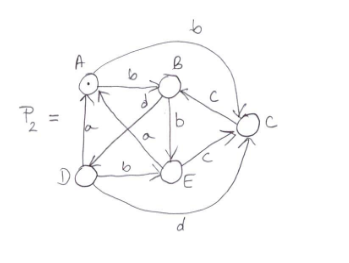
\includegraphics{./imgs/Question-2-a-ii.png}
	\caption{Question 2-a LTS 2}
	\label{fig:Question-2-a-ii-LTS}
\end{figure}

\begin{figure}[H]
	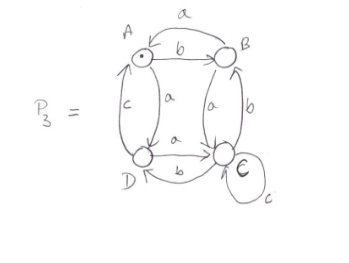
\includegraphics{./imgs/Question-2-a-iii.png}
	\caption{Question 2-a LTS 3}
	\label{fig:Question-2-a-iii-LTS}
\end{figure}

\subsection[~\thesubsection]{For each of the following three processes, give an FSP description of the labelled transition graph. Dots indicate initial states.}

\subsubsection[~\thesubsubsection]{FSP Description for P1}

\begin{align*}
	\text{A} &= (\text{a} \rightarrow \text{B} \; | \; \text{a} \rightarrow \text{D}) \\
	\text{B} &= (\text{b} \rightarrow \text{C} \; | \; \text{c} \rightarrow \text{D}) \\
	\text{C} &= ((\text{a} \rightarrow \text{D} \; | \; \text{b} \rightarrow \text{A}) \; | \; \text{d} \rightarrow \text{C}) \\
	\text{D} &= (\text{d} \rightarrow \text{A})
\end{align*}

\subsubsection[~\thesubsubsection]{FSP Description for P2}

\begin{align*}
	\text{A} &= (\text{b} \rightarrow \text{B} \; | \; \text{b} \rightarrow \text{C}) \\
	\text{B} &= (\text{b} \rightarrow \text{E} \; | \; \text{d} \rightarrow \text{d}) \\
	\text{C} &= (\text{c} \rightarrow \text{B}) \\
	\text{D} &= ((\text{a} \rightarrow \text{A} \; | \; \text{d} \rightarrow \text{C}) \; | \; \text{b} \rightarrow \text{E}) \\
	\text{E} &= (\text{a} \rightarrow \text{A} \; | \; \text{c} \rightarrow \text{C})
\end{align*}

\subsubsection[~\thesubsubsection]{FSP Description for P2}

\begin{align*}
	\text{A} &= (\text{a} \rightarrow \text{D} \; | \; \text{b} \rightarrow \text{B}) \\
	\text{B} &= (\text{a} \rightarrow \text{A} \; | \; \text{a} \rightarrow \text{C}) \\
	\text{C} &= ((\text{b} \rightarrow \text{B} \; | \; \text{b} \rightarrow \text{D}) \; | \; \text{c} \rightarrow \text{C}) \\
	\text{D} &= (\text{a} \rightarrow \text{C} \; | \; \text{c} \rightarrow \text{A})
\end{align*}

\subsection[~\thesubsection]{Use an LTSA tool to transform your FSPs back into LTSs. Compare the results and discuss any differences.}

\begin{figure}[H]
	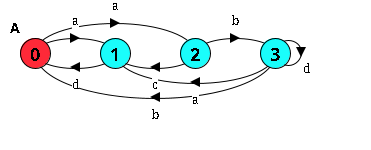
\includegraphics{./imgs/Question-2-b-i.png}
	\caption{Question 2-b LTS 1}
	\label{fig:Question-2-b-i-LTS}
\end{figure}

\begin{figure}[H]
	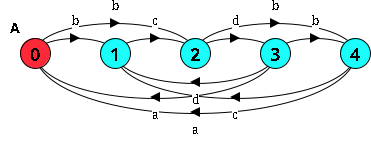
\includegraphics{./imgs/Question-2-b-ii.png}
	\caption{Question 2-b LTS 2}
	\label{fig:Question-2-b-ii-LTS}
\end{figure}

\begin{figure}[H]
	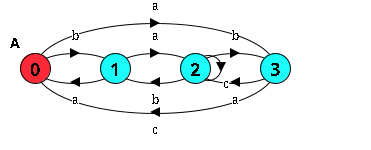
\includegraphics{./imgs/Question-2-b-iii.png}
	\caption{Question 2-b LTS 3}
	\label{fig:Question-2-b-iii-LTS}
\end{figure}

Each of the LTSs produced by the LTS tool are functionally equivalent to the ones given in the question, apart from the fact that the states are numbered rather than labelled alphabetically and arranged horizontally. In the code I used to produce the LTSs, the only difference of note compares to the FSPs I derived was that I had to unnest choices whenever I nested them to get it to compile.

\section[Question ~\thesection]{A miniature portable FM radio has three controls. An on/off switch which turns the device on and off. Tuning is controlled by two buttons: Scan and reset. When the device is turned on or reset is pressed, the radio is tuned to the top freqyency of the FM band (108MHz). When scan is pressed, the radio scans towards the bottom of the band (88MHz), It stops scanning when it locks onto a station or it reaches the bottom (end). If the radio is currently tuned to a station and scan is pressed, it starts to scan from the frequency of that station towards the bottom. Similarly, when reset is pressed, the receiver tunes to the top. Model the radio as an FSP (RADIO) and provide an appropriate LTS. (Hint: The alphabet of RADIO is \{on, off, reset, lock, end\}).}

\subsection{}

\subsubsection[~\thesubsubsection]{FSP Description}

\begin{align*}
	\text{RADIO} &= OFF \\
	\text{OFF} &= (\text{on} \rightarrow \text{TOP}) \\
	\text{TOP} &= (\text{scan} \rightarrow \text{SCAN}\; | \; \text{reset} \rightarrow \text{TOP} \; | \; \text{lock} \rightarrow \text{ON} \; | \; \text{off} \rightarrow \text{OFF}) \\
	\text{ON} &= (\text{scan} \rightarrow \text{SCAN} \; | \; \text{reset} \rightarrow \text{ON} \; | \;\text{off} \rightarrow \text{OFF} \; | \; \text{lock} \rightarrow \text{ON}) \\
	\text{SCAN} &= (\text{lock} \rightarrow \text{ON} \; | \; \text{end} \rightarrow \text{BOTTOM} \; | \; \text{reset} \rightarrow \text{TOP} \; | \; \text{off} \rightarrow \text{OFF}) \\
	\text{BOTTOM} &= (\text{scan} \rightarrow \text{SCAN} \; | \; \text{reset} \rightarrow \text{TOP} \; | \; \text{off} \rightarrow \text{OFF})
\end{align*}

\subsubsection[~\thesubsubsection]{LTS Representation}

\begin{figure}[H]
	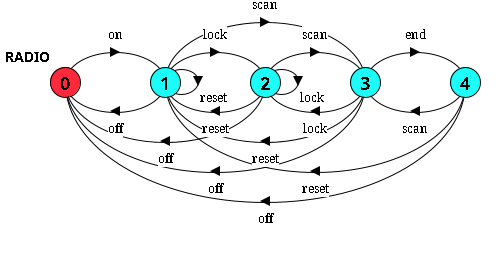
\includegraphics{./imgs/Question-3.png}
	\caption{Question 3 LTS Generated by LTSA}
	\label{fig:Question-2-b-iii-LTS}
\end{figure}

\section[Question ~\thesection]{Program the radio in Question 3 in Java, complete with a graphic display (if possible)}

Code provided in appendix

\section[Question ~\thesection]{A drinks Machine machine charges 15\textcent $\,$ for a can of Sugarola, 20\textcent $\,$ for a can of SugarolaDiet, and 25\textcent $\,$ for a can of SugarolaSuperDiet. The machine accepts 5\textcent, 10\textcent, and 25\textcent $\,$ denomination coins and provides change. Model the machine as an FSP process, DRINKS.}

\begin{align*}
	\text{const SUGAROLA} &= 15 \\
	\text{const DIET} &= 20 \\
	\text{const SUPERDIET} &= 25 \\
	\text{range CREDIT} &= 0..25 \\
	\text{DRINKS} &= \text{CREDIT[0]}, \\
	\text{CREDIT[c:CREDIT]} &= (\text{when} (c + 5 \le 25) \text{nickel} \rightarrow \text{CREDIT[c+5]} \\
	&| \text{when} (c + 10 \le 25) \text{dime} \rightarrow \text{CREDIT[c+10]} \\
	&| \text{when} (c \ge \text{SUGAROLA}) \text{sugarola} \rightarrow \text{CHANGE[c-SUGAROLA]} \\
	&| \text{when} (c \ge \text{DIET}) \text{diet} \rightarrow \text{CHANGE[c-DIET]} \\
	&| \text{when} (c \ge \text{SUPERDIET}) \text{superdiet} \rightarrow \text{CHANGE[c-SUPERDIET]}
	), \\
	\text{CHANGE[r:CREDIT]} &= (\text{when} (r \ge 10)\text{change10} \rightarrow \text{CHANGE[r-10]} \\
	&| \text{when} (r \ge 5) \text{change5} \rightarrow \text{CHANGE[r-5]} \\
	&| \text{CREDIT[0]}.
\end{align*}

\section[Question ~\thesection]{Consider the following set of FSPs}

\begin{align*}
	\text{A} &= (((\text{a} \rightarrow (\text{b} \rightarrow \text{A})) \; | \; (\text{c} \rightarrow (\text{a} \rightarrow \text{C} \; | \; \text{c} \rightarrow \text{B})) \; | \; (\text{c} \rightarrow \text{C}))) \\
	\text{B} &= (\text{b} \rightarrow (\text{a} \rightarrow \text{B} \; | \; \text{c} \rightarrow (\text{a} \rightarrow \text{A} \; | \; \text{b} \rightarrow \text{B}))) \\
	\text{C} &= ((\text{a} \rightarrow (\text{b} \rightarrow (\text{c} \rightarrow \text{B}))) \; | \; (\text{a} \rightarrow \text{C}))
\end{align*}

\subsection[~\thesubsection]{Construct an equivalent LTS using the rules from page 16 of lecture notes 2}

\begin{figure}[H]
	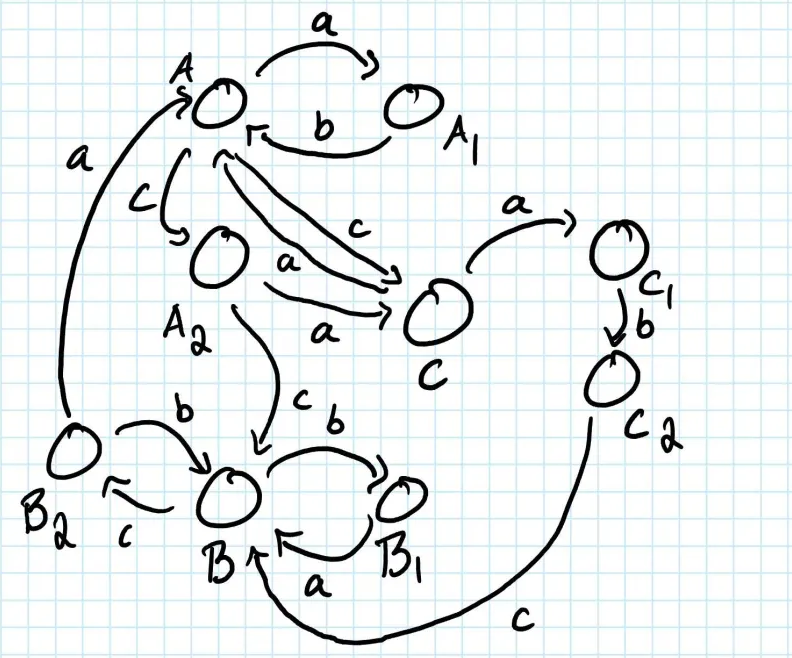
\includegraphics[width=\linewidth]{./imgs/Question-6-a.png}
	\caption{Question 6-a LTS made by me}
	\label{fig:Question-6-a}
\end{figure}

\subsection[~\thesubsection]{Use an LTSA tool to produce an appropriate LTS. If it differs from yours, analyse and explain those differences.}

\begin{figure}[H]
	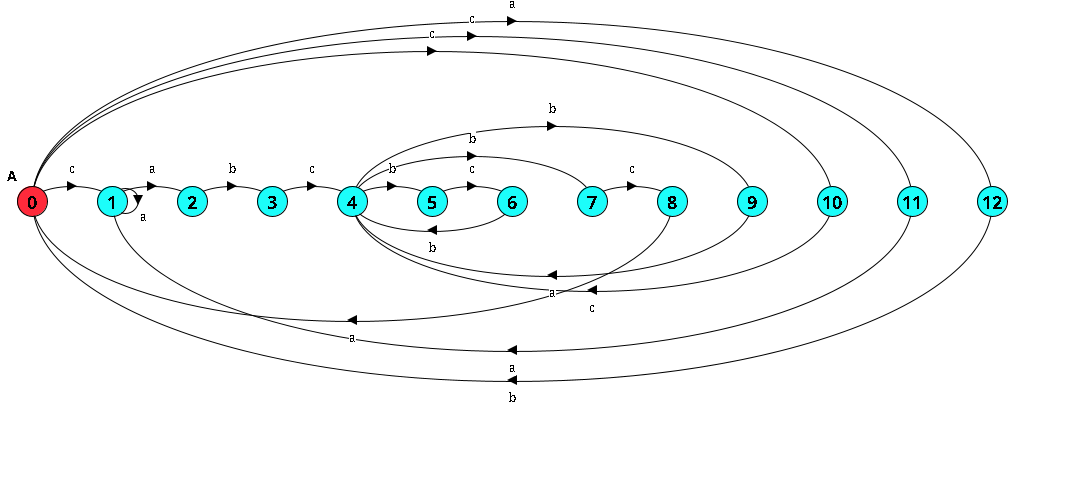
\includegraphics[width=\linewidth]{./imgs/Question-6-b.png}
	\caption{Question 6-b LTS made by LTSA}
	\label{fig:Question-6-b}
\end{figure}

The solution I produced does differ from the one produced by the LTSA tool in the sense that the LTSA tool used more states to represent the behaviour of the FSP (13) than I did (9). However, both LTSs are functionally equivalent. I suspect the reason why the LTSA tool produced more states is because it chose to always create a new state every time a there existed a nested transition, whereas I chose to reuse states where ever possible to produce a slightly more concise, although equivalent, LTS.

\section[Question ~\thesection]{Consider the following two processes, $||$S1 and S2:}

\begin{align*}
	\text{P} &= (\text{a} \rightarrow \text{b} \rightarrow \text{d} \rightarrow {P}) \\
	\text{Q} &= (\text{c} \rightarrow \text{b} \rightarrow \text{e} \rightarrow {Q}) \\
	||\text{S1} &= (\text{P} \; || \; \text{Q})
\end{align*}

\subsection[~\thesubsection]{Show that the processes $||$S1 and S2 generate the same LTSs. I.e. LTS($||$S1) = LTS(S2) (or equivalently, they exhibit the same behaviour)}

Using an LTSA tool, we can see that $||$S1 and S2 generate LTSs which produce the exact same traces. Thus, we can see that their behaviour must be equivalent. You can see the generated LTSs below:

\begin{figure}[H]
	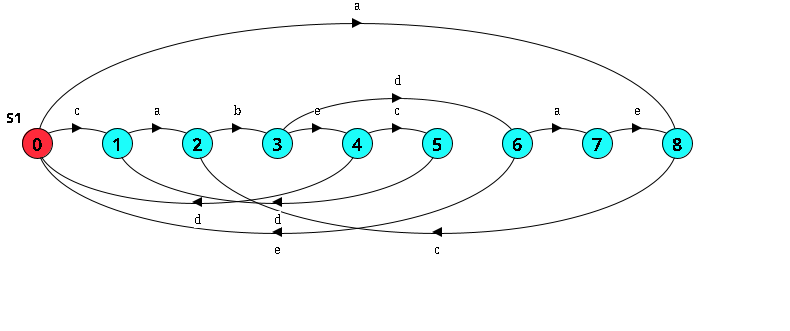
\includegraphics[width=\linewidth]{./imgs/Question-7-i.png}
	\caption{LTS for $||$S1 for Question 7}
	\label{fig:Question-7-i}
\end{figure}

\begin{figure}[H]
	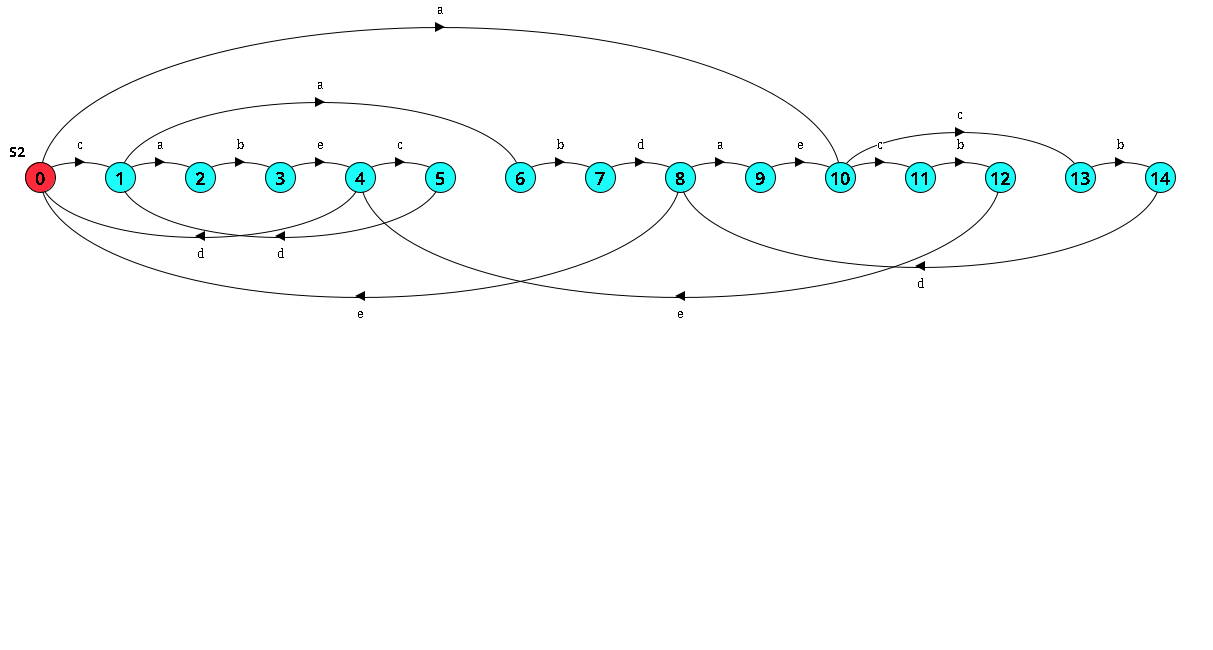
\includegraphics[width=\linewidth]{./imgs/Question-7-ii.png}
	\caption{LTS for S2 for Question 7}
	\label{fig:Question-7-ii}
\end{figure}

\subsection[~\thesubsection]{Using a method presented on page 17 of Lecture Notes 3 and pages 10-11 of Lecture Notes 4, transform the processes $||$S1 and S2 into appropriate Petri nets. Are these nets identical? Explain the differences. Which one allows simultaneity?}

\begin{figure}[H]
	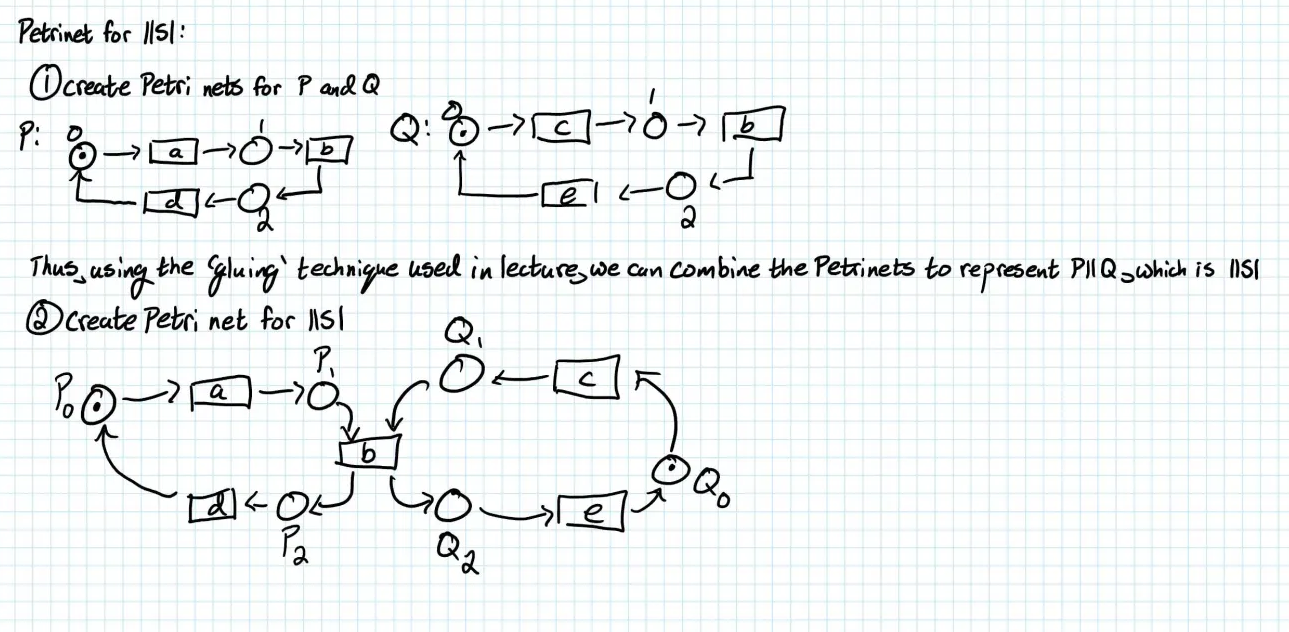
\includegraphics[width=\linewidth]{./imgs/Question-7-b-i.png}
	\caption{Petri net for $||$S1 for Question 7}
	\label{fig:Question-7-b-i}
\end{figure}

\begin{figure}[H]
	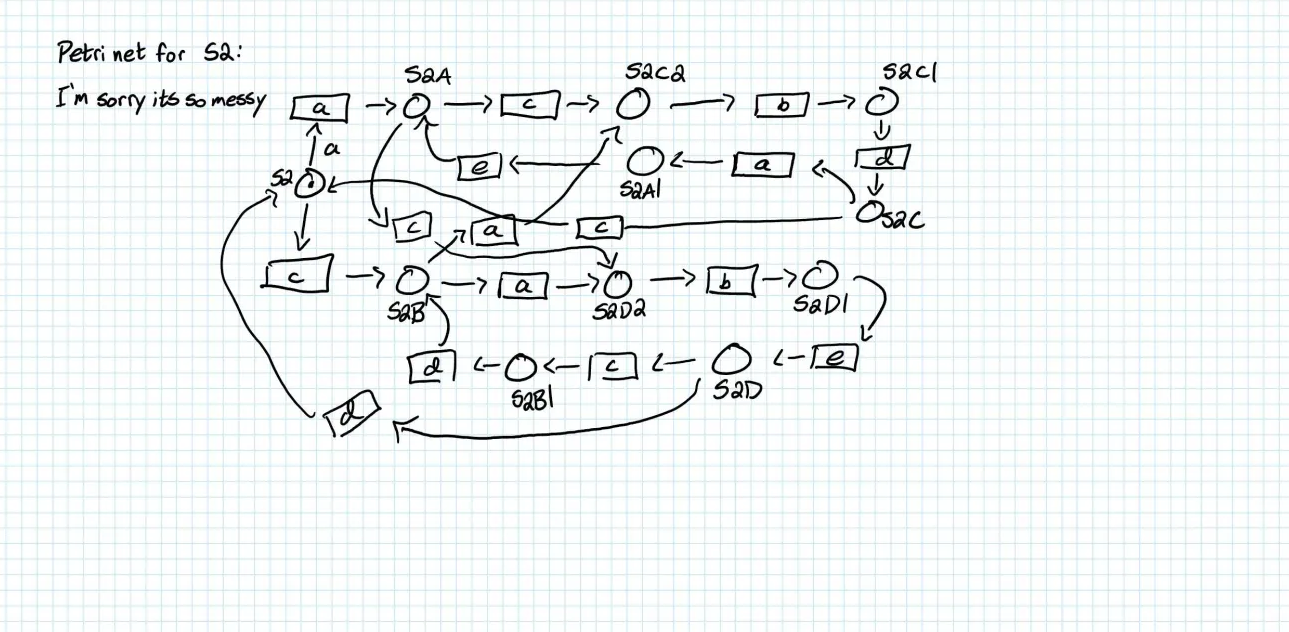
\includegraphics[width=\linewidth]{./imgs/Question-7-b-ii.png}
	\caption{Petri net for S2 for Question 7}
	\label{fig:Question-7-b-ii}
\end{figure}

The nets are clearly not identical. Superficially, the net for $||$S1 is much simpler with far fewer places and transitions than S2, however, we can also notice that the net for $||$S1 contains two, rather than a single, initial token, and has a transition (the b transition) which is shared by different places, whereas S2 does not. Due to the fact $||$S1 has multiple tokens, only $||$S1 allows is capable of modelling simultaneity.

\section[Question ~\thesection]{Model the Petri net $N_1$ (given below) as the composition of FSP processes}

\begin{figure}[H]
	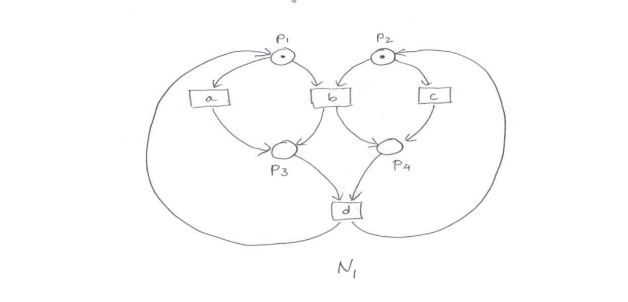
\includegraphics[width=\linewidth]{./imgs/Question-8.png}
	\caption{Petri net for Question 8}
	\label{fig:Question-8}
\end{figure}

We can model $N_1$ with the following FSP:

\begin{align*}
	P_1 &= (\text{a} \rightarrow \text{d} P_1 \; | \; \text{b} \rightarrow \text{d} \rightarrow P_1) \\
	P_2 &= (\text{c} \rightarrow \text{d} P_2 \; | \; \text{b} \rightarrow \text{d} \rightarrow P_2) \\
	||N_1 &= (P_1||P_2)
\end{align*}

\section[Question ~\thesection]{Model the system from page 10 of lecture notes 3 as the composition of FSP processes. The entities represented by places in the Petri net model must be represented as actions/transitions in the FSP model}

The Petri-net in the slide is given by:

\begin{figure}[H]
	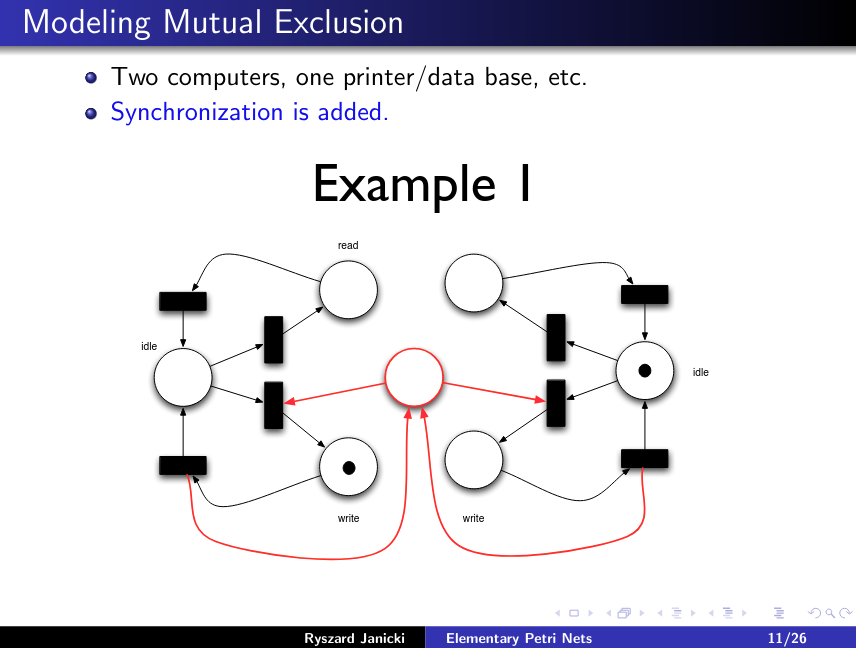
\includegraphics[width=\linewidth]{./imgs/Question-9.png}
	\caption{Petri net for Question 9}
	\label{fig:Question-9}
\end{figure}

We can describe this system (denoted SYSTEM) by the parallel composition of the processes LOCK, EXECUTE, and PAUSE. The FSP for this system is given below:

\begin{align*}
	\text{LOCK} &= (\text{acquire} \rightarrow \text{release} \rightarrow \text{LOCK}) \\
	\text{EXECUTE} &= (\text{read} \rightarrow \text{PAUSE} \; | \; \text{acquire} \rightarrow \text{write} \rightarrow \text{release} \rightarrow \text{PAUSE}) \\
	\text{PAUSE} &= (\text{idle} \rightarrow \text{EXECUTION}) \\
	||\text{SYSTEM} &= (\text{LOCK}||\text{EXECUTE}||\text{PAUSE})
\end{align*}

\section[Question ~\thesection]{A roller coaster control system only permits its car to depart when it's full. Passengers arriving at the departure platform are registered with the roller-coaster controller by a turnstile. The controller signals the car to depart when there are enough passengers on the platform to fill the car to its maximum capacity of M passengers. Ignore the synchronization detail of passengers embarking from the platform and car departure. The roller-coaster consists of three processes: TURNSTILE, CONTROL, and CAR. TURNSTILE and CONTROL interact by the shared action 'passenger' indicating the arrival of a passenger. CONTROL and CAR interact by the shared action 'depart' which signals the car to depart. Provide an FSP description of each process and the overall composition.}

Since we're not given what the actual maximum capacity of the car is, I'm referencing it ambiguously in the FSP. In an actual implementation, all we would need to do is just substitute \emph{some\_number} with an integer.

\begin{align*}
\text{MAXIMUM\_CAPACITY} &= \textit{some\_number} \\
\text{TURNSTILE} &= (\text{passenger} \rightarrow \text{TURNSTILE}) \\
\text{CAR} &= (\text{depart} \rightarrow \text{CAR}) \\
\text{CONTROL} &= \text{CONTROL[0]} \\
\text{CONTROL}[i:0..\text{MAXIMUM\_CAPACITY}] &= 
  (\text{when } i < \text{MAXIMUM\_CAPACITY}) \ \text{passenger} \rightarrow \text{CONTROL}[i+1] \\
&\mid (\text{when } i = \text{MAXIMUM\_CAPACITY}) \ \text{depart} \rightarrow \text{CONTROL}[0] \\
||\text{RIDE} &= (\text{TURNSTILE} \;||\; \text{CONTROL} \;||\; \text{CAR})
\end{align*}

\section[Question ~\thesection]{Construct a reachability graph (defined on page 18 of lecture notes 3) for the Petri net given in Question 8.}

From Question 8, we were able to determine that the Petri net can be described by the FSP:

\begin{align*}
	P_1 &= (\text{a} \rightarrow \text{d} P_1 \; | \; \text{b} \rightarrow \text{d} \rightarrow P_1) \\
	P_2 &= (\text{c} \rightarrow \text{d} P_2 \; | \; \text{b} \rightarrow \text{d} \rightarrow P_2) \\
	||N_1 &= (P_1||P_2)
\end{align*}

Drawing this out, we can see that $P_1$ and $P_2$ are given by the LTSs:

\begin{figure}[H]
	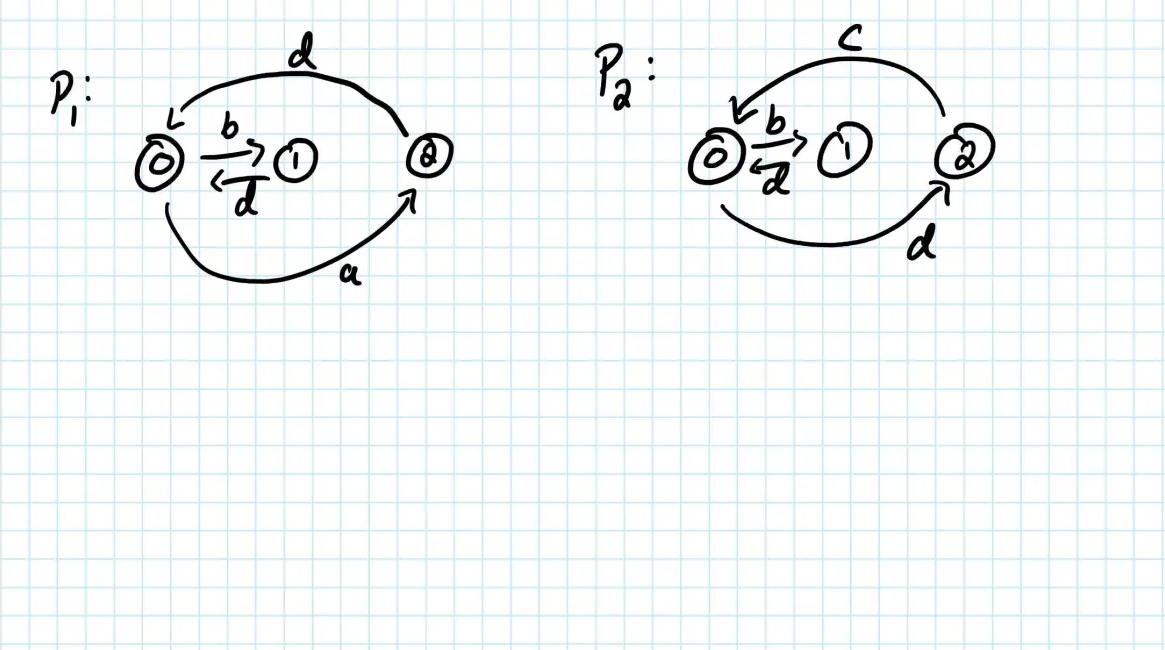
\includegraphics[width=\linewidth]{./imgs/Question-9-LTSs.png}
	\caption{LTSs for Question 9}
	\label{fig:Question-9}
\end{figure}

Using this, we can take the cross product of the states in each LTS to arrive at the reachability graph for $N_1$:

\begin{figure}[H]
	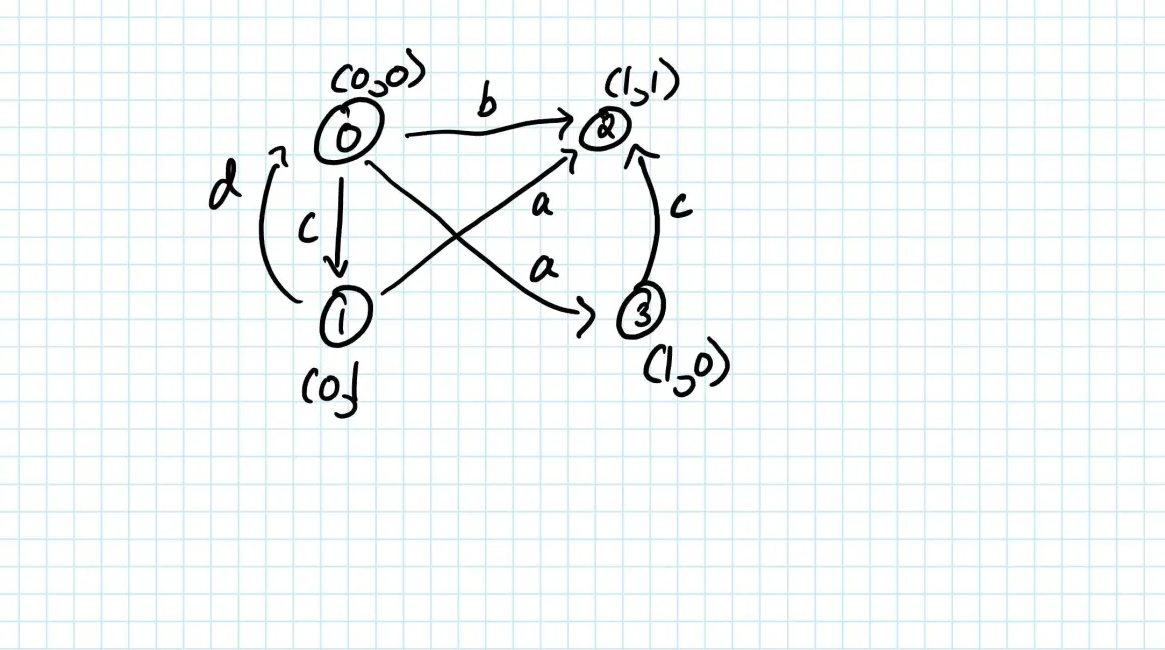
\includegraphics[width=\linewidth]{./imgs/Question-9-Reachability-Graph.png}
	\caption{Reachability graph for Question 9}
	\label{fig:Question-9}
\end{figure}

\section[Question ~\thesection]{Consider the three LTSs given below, $P_1, P_2$, and $P_3$ (where tokens represent initial states):}

\begin{figure}[H]
	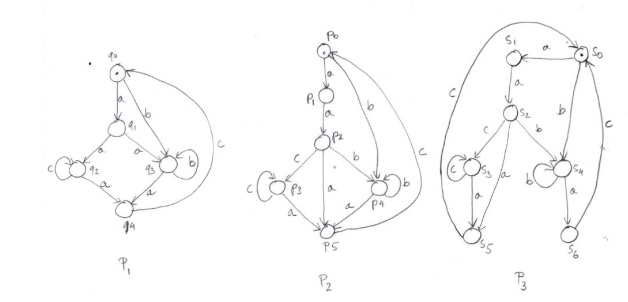
\includegraphics[width=\linewidth]{./imgs/Question-12.png}
	\caption{LTSs for Question 12}
	\label{fig:Question-12}
\end{figure}

\subsection[~\thesubsection]{Show that $P_2 \approx P_3$ ($P_2$ and $P_3$ are bisimilar)}

By definition of bisimilarity, we know that $P_1$ and $P_3$ are bisimilar if all states in $P_2$ reachable by some trace from the initial state is bisimilar to all states reachable by the same trace in $P_3$. Using this definition, we can see that:

\begin{itemize}
	\item $p_0 \approx s_0$ since they are both initial states (reachable by the zero-length string) and can both execute the action 'a'.
	\item $p_1 \approx s_1$ since they are both reachable by the trace 'a' and both can execute the 'a' action.
	\item $p_2 \approx s_2$ since both $p_2$ and $s_2$ are reachable by the trace 'aa' and both can execute the 'a', 'b', and 'c' actions.
	\item $p_3 \approx s_3$ since $p_3$ and $s_3$ are both reachable by the trace 'aac' and both can execute the 'a' and 'c' actions.
	\item $p_4 \approx s_4$ since both are reachable by the traces 'aab' and 'b' and both can execute the 'a' and 'b' actions.
	\item $p_5 \approx s_4$ and $s_6$. We know that $p_5$ is reachable by the traces 'aaa', 'aacc*a', 'bb*a', and 'aaa'. As for $s_5$ and $s_6$, we know $s_5$ is reachable by 'aacc*a' and 'aaa' and $s_6$ is reachable by the traces 'bb*a' and 'aab*a'. Thus, all traces from the initial state that reach $p_5$ also reach either $s_5$ or $s_6$. Now since, $p_5$ can execute actions 'c', and $s_5$ and $s_6$ can also execute 'c', the same set of actions can be executed for the same traces, this making $p_5$ bisimilar to both $s_5$ and $s_6$.
\end{itemize}

Therefore, since all states in $P_2$ are bisimilar to all states reachable by the same trace in $P_3$, $P_2$ and $P_3$ are bisimilar and thus $P_2 \approx P_3$.

\subsection[~\thesubsection]{Show that $P_1 \not\approx P_2$ ($P_1$ and $P_2$ are NOT bisimilar)}

We can prove that $P_1$ and $P_2$ are not bisimilar by simply illustrating a single example of a trace in $P_1$ which leads to a state in $P_1$ which isn't bisimilar to any state in $P_2$ with the same trace.

Consider the trace 'a' in $P_1$. This leads us to a state $q_1$. $q_1$ is capable of \underline{non-deterministically} executing the action a, leading to two different states in $P_1$ ($q_2$ and $q_3$). The same trace, 'a', leads us to state $p_1$ in $P_2$, which is only capable of deterministically executing a single 'a' transition. Therefore, since two states reachable by the same trace ('a') are not bisimilar, then $P_1$ and $P_2$ are not bisimilar and thus $P_1 \not\approx P_2$.

\subsection[~\thesubsection]{Show that $P_1 \not\approx P_3$ ($P_1$ and $P_3$ are NOT bisimilar)}

We can prove that $P_1$ and $P_3$ are not bisimilar by the same methedology as earlier.

Consider once again the trace 'a' in $P_1$. This takes us to the state $q_1$, which as stated before, can non-deterministically execute action 'a' and lead to states $q_2$ and $q_3$ in $P_1$. The trace 'a' in $P_3$ leads to state $s_1$ which only has a single, deterministic 'a' transition leading to a single other state, $s_2$. Therefore, these two states, which are reachable by the same trace, are not bisimilar, $P_1$ and $P_3$ are not bisimilar and thus $P_1 \not\approx P_3$.

\subsection[~\thesubsection]{Show that Traces($P_1$) = Traces($P_2$) = Traces($P_3$) = Pref(\emph{Some regular expression})}

\subsubsection[~\thesubsubsection]{Traces($P_1$)}
To find all the traces of $P_1$ we must find the set of all traces which return us to the initial state. The trace 'a' takes us to the state $q_1$ from $q_0$ (our initial state). From $q_1$, we can non-deterministically take 'a' to either $q_2$ or $q_3$ (making our current trace 'aa'). At $q_2$, we can execute $c$ an indefinite number of times while remaining at $q_2$ or take an 'a' transition to $q_4$. At $q_3$, we can similarly execute 'b' an indefinite number of times or take an 'a' transition to end up at state $q_4$. Thus, $q_4$ is reachable by the traces (aab*a|aac*a). $q_4$ connects us back to our initial state with the 'c' transition and therefore (aa(b*|c*)ac)* is a set of traces of $P_1$. However, there also exists a 'b' transition connecting $q_0$ to $q_3$, and using our prior knowledge of $q_3$, we can ascertain that the set of all traces of $P_1$ is given by Pref(((aa(c*|b*)|(bb*))ac)*).

\subsubsection[~\thesubsubsection]{Traces($P_2$)}
We use the same strategy as before to ascertain the traces of $P_2$. The trace 'a' takes us from the initial state $p_0$ to $p_1$ and taking 'a' again leads us to $p_2$, giving us out current trace of 'aa'. From $p_2$, we can take either an 'a', 'b', or 'c' transition to the states $p_5$, $p_4$, or $p_3$ respectively. Taking the 'b' transition to $p_4$, we can take the 'b' transition an indefinite number of times, remaining at $p_4$ or take an 'a' transition to $p_5$. Similarly, from $p_3$ we can take a c transition an indefinite number of times befre transitioning to $p_5$ by executing 'a'. Thus the traces 'aaa', 'aacc*a', and 'aabb*a' all take us to $p_5$. Since $p_5$ takes us back to the initial state with a 'c' transition, we know (aa(cc*|bb*)ac)* are all traces of our system. However, there also exists a 'b' transition frm $p_0$ to $p_4$, and using our knowledge of $p_4$, we can therefore conclude that the set of all traces of $P_2$ can be given by Pref(((aa(c*|b*)|(bb*))ac)*).

\subsubsection[~\thesubsubsection]{Traces($P_3$)}
Using the same process, we see that 'a' takes us from $s_0$ to $s_1$, and another 'a' moves us from $s_1$ to $s_2$. From $s_2$, we can take an 'a', 'b', or 'c' transition to states $s_5$, $s_4$, or $s_3$ respectively. At $s_3$, we can take a 'c' transition an indefinite number of times, remaining at $s_3$, before taking an 'a' transition to $s_5$. Likewise, at $s_4$, we can take the 'b' transition an indefinite number of times before taking an 'a' transition to $s_6$. From both $s_5$ and $s_6$, we can take a 'c' transition to return back to our initial state $s_0$. However, we can also take a 'b' transition directly from $s_0$ to $s_4$, and using our prior description of $s_4$, we can conclude that the traces of $P_3$ is given by Pref(((aa(c*|b*)|(bb*))ac)*).

Thus, the traces of $P_1$, $P_2$, and $P_3$ are all equivalent and given by Pref(((aa(c*|b*)|(bb*))ac)*).

\section{Appendix}

\subsection{Question 1 LTSA Code}

\begin{lstlisting}
REQUEST = (room_available -> confirm -> CHOICE | room_unavailable -> wait -> WAITLIST),
CHOICE = (use -> pay -> leave -> archive -> STOP | cancel -> STOP),
WAITLIST = (room_available -> confirm -> CHOICE | room_unavailable -> WAIT),
WAIT = (cancel -> STOP | wait -> WAITLIST).
\end{lstlisting}

\subsection{Question 2 LTSA Code}

\subsubsection{}

\begin{lstlisting}
A = (a -> B | a -> D),
B = (b -> C | c -> D),
C = (a -> D | b -> A | d -> C),
D = (d -> A).
\end{lstlisting}

\subsubsection{}

\begin{lstlisting}
A = (b -> B | b -> C),
B = (b -> E | d -> D),
C = (c -> B),
D = (a -> A | d -> C | b -> E),
E = (a -> A | c -> C).
\end{lstlisting}

\subsubsection{}

\begin{lstlisting}
A = (a -> D | b -> B),
B = (a -> A | a -> C),
C = (b -> B | b -> D | c -> C),
D = (a -> C | c -> A).
\end{lstlisting}

\subsection{Question 3 LTSA Code}

\begin{lstlisting}
RADIO = OFF,

OFF = (on -> ON_TOP),

ON_TOP = (scan -> SCANNING
         | reset -> ON_TOP
         | off -> OFF
         | lock -> ON_STATION),

ON_STATION = (scan -> SCANNING
             | reset -> ON_TOP
             | off -> OFF
             | lock -> ON_STATION),

SCANNING = (lock -> ON_STATION
           | end -> ON_BOTTOM
           | reset -> ON_TOP
           | off -> OFF),

ON_BOTTOM = (scan -> SCANNING
            | reset -> ON_TOP
            | off -> OFF).

\end{lstlisting}

\subsection{Question 4 Java Code}

\begin{lstlisting}
import javax.swing.*;
import java.awt.*;

public class RadioSimulator extends JFrame {
    enum State { OFF, ON_TOP, ON_STATION, SCANNING, ON_BOTTOM }
    private State state = State.OFF;
    private JLabel display;
    private int frequency = 108;
    private Timer scanTimer;

    public RadioSimulator() {
        super("Mini FM Radio");
        display = new JLabel("State: OFF", SwingConstants.CENTER);
        display.setFont(new Font("Arial", Font.BOLD, 20));
        add(display, BorderLayout.CENTER);

        JPanel buttons = new JPanel(new GridLayout(1, 5));
        JButton onBtn = new JButton("On");
        JButton offBtn = new JButton("Off");
        JButton scanBtn = new JButton("Scan");
        JButton resetBtn = new JButton("Reset");
        JButton lockBtn = new JButton("Lock");
        buttons.add(onBtn);
        buttons.add(offBtn);
        buttons.add(scanBtn);
        buttons.add(resetBtn);
        buttons.add(lockBtn);
        add(buttons, BorderLayout.SOUTH);

        scanTimer = new Timer(300, e -> {
            if (state == State.SCANNING) {
                if (frequency > 88) {
                    frequency--;
                } else {
                    state = State.ON_BOTTOM;
                    scanTimer.stop();
                }
                update();
            }
        });

        onBtn.addActionListener(e -> {
            if (state == State.OFF) {
                state = State.ON_TOP;
                frequency = 108;
            }
            update();
        });
        offBtn.addActionListener(e -> {
            state = State.OFF;
            scanTimer.stop();
            update();
        });
        scanBtn.addActionListener(e -> {
            if (state == State.ON_TOP || state == State.ON_STATION || state == State.ON_BOTTOM) {
                state = State.SCANNING;
                scanTimer.start();
            }
            update();
        });
        resetBtn.addActionListener(e -> {
            if (state != State.OFF) {
                state = State.ON_TOP;
                frequency = 108;
                scanTimer.stop();
            }
            update();
        });
        lockBtn.addActionListener(e -> {
            if (state == State.SCANNING) {
                state = State.ON_STATION;
                scanTimer.stop();
            }
            update();
        });

        setSize(400, 200);
        setDefaultCloseOperation(EXIT_ON_CLOSE);
        setVisible(true);
    }

    private void update() {
        if (state == State.OFF) display.setText("State: OFF");
        else display.setText("State: " + state + "  Frequency: " + frequency + " MHz");
    }

    public static void main(String[] args) {
        SwingUtilities.invokeLater(RadioSimulator::new);
    }
}
\end{lstlisting}

\subsection{Question 6 LTSA Code}

\begin{lstlisting}
A = (a-> b -> A | c -> a -> C | c -> c -> B | c -> C),
B = (b -> a -> B | b -> c -> a -> A | b -> c -> b -> B),
C = (a -> b -> c -> B | a -> C).
\end{lstlisting}

\subsection{Question 7 LTSA Code}

\subsubsection{}

\begin{lstlisting}
P = ( a -> b -> d -> P).
Q = ( c -> b -> e -> Q ).
||S1 = (P||Q).
\end{lstlisting}

\subsubsection{}

\begin{lstlisting}
S2 = ( a -> S2A | c -> S2B ),
S2A = ( c -> b -> d -> S2C | c -> b -> e -> S2D ),
S2B = ( a -> b -> d -> S2C | a -> b -> e -> S2D ),
S2C = ( e -> S2 | a -> e -> S2A ),
S2D = ( d -> S2 | c -> d -> S2B ).
\end{lstlisting}

\end{document}
